\documentclass[10pt]{beamer}

%%%
% PREAMBLE FOR THIS DOC 
%%%
%https://tex.stackexchange.com/questions/68821/is-it-possible-to-create-a-latex-preamble-header
\usepackage{/Users/miw267/Repos/csci246_spring2025/slides/preambles/beamer_preamble_for_CSCI246}



%%% TRY TO RESHOW TOC AT EACH SECTION START (with current section highlighted)
% Reference: https://tex.stackexchange.com/questions/280436/how-to-highlight-a-specific-section-in-beamer-toc
\newcommand\tocforsect[2]{%
  \begingroup
  \edef\safesection{\thesection}
  \setcounter{section}{#1}
  \tableofcontents[#2,currentsection]
  \setcounter{section}{\safesection}
  \endgroup
}


%%%% HERES HOW TO DO IT CORRECTLY
% FIRST IN .STY FILE, DO
%\usetheme[sectionpage=none]{metropolis}
% THEN AT EACH SECTION DO
%\begin{frame}{Outline}
%  \tableofcontents[currentsection]	
%\end{frame}



%\setbeamertemplate{navigation symbols}{}
%\setbeamertemplate{footline}[frame number]{}


%%%
% DOCUMENT
%%%

\begin{document}

%\maketitle

%% Title page frame
%\begin{frame}
%    \titlepage 
%\end{frame}





\title{Friday 01/24/2025: Counterexample}
\author{CSCI 246: Discrete Structures}
\date{Textbook reference: Sec. 6, Scheinerman}

\begin{frame}
    \titlepage 
\end{frame}


\begin{frame}


\begin{mygreenbox}[title=Quiz Set up]
\begin{itemize}
\item \textbf{Sheet of paper}: Please bring your own sheet of paper to class each day for quizzes if possible. However, if you don't have any, you are welcome to take a blank sheet of paper from the stack in the front of the room.
\item \textbf{Rules for quizzes}: For all quizzes in the course, you should use only paper and pencil.  Please close your computers and textbooks, and put away your cellphones.    
\end{itemize}
\end{mygreenbox}


\begin{myyellowbox}[title=Today's Agenda]
\begin{itemize}
	\item Reading quiz / problems quiz (10 mins)
	\item Mini-lecture ($\approx$ 15 mins)
	%
	\begin{itemize}
	\item Go over Sec. 5 group problems
	\item Comments on Sec. 5 reading quiz
	\end{itemize}
	%
	\item Group exercises ($\approx$ 25 mins)	
\end{itemize}

\end{myyellowbox}



\end{frame}






\begin{frame}{Friday Quiz}


 \begin{mygreenbox}[title=Reading Quiz (Sec. 6 - Counterexamples)]
Disprove the following conjecture: \\
\vfill 
\textit{Let $a$ and $b$ be integers.  If $a|b$ and $b|a$, then $a=b$.}  \\
\vfill 
Note: You can disprove the conjecture by providing a counterexample.  Make sure to show that your counterexample satisfies the hypothesis (the "if" statement), but not the conclusion (the "then" statement).
\vfill 
\end{mygreenbox}

\vfill \vfill 


 \begin{mygreenbox}[title=Problems Quiz (Sec. 4 - Theorems)]
Two propositions are considered \textit{equivalent} if they have the same truth table values.  Show that the biconditional $A \iff B$ is equivalent to $(A \implies B) \, \texttt{and} \, (B \implies A)$.
\end{mygreenbox}
\end{frame}

\section{Mini-lecture}

\begin{frame}[standout]

\vfill 
\alert{Review solutions to Sec. 5 group exercises}
\vfill

\end{frame}


\begin{frame}{Observation on Sec. 5 (Proofs) reading quiz}

\begin{myyellowbox}[title=\textbf{Observation}] 
A number of students wrote out expressions that look something like
\[ 2|x + 2|y = 2|z\]
\end{myyellowbox}

\begin{myredbox}[title=\textbf{Warning}] 
This expression has no meaning.    Note from the definition of divisibility (see below) that $2|x$ is itself \textit{already} an equation.  The notation $2|x$  \textit{means} that there is an integer $a$ such that $2a=x$.	
\end{myredbox}


\vfill 
\begin{mydef}[title=Definition (\textbf{Divisible})]
Let $a$ and $b$ be integers.  We say that $a$ is \textit{divisible} by $b$ (notated as $b|a$) provided there is an integer $c$ such that $bc=a$.  
\end{mydef}


\end{frame}


\begin{frame}{How I graded the reading quiz for Sec. 5 (Proofs)}
\textbf{Proposition.} The sum of two even integers is even.

\textbf{Proof.}

\begin{tabularx}{\textwidth}{|L{1cm}|L{3cm}|X|}
\hline 
\textbf{Points} & \textbf{Role} & \textbf{Text} \\ \hline
 & \hlorange{Convert Prop. to ``if-then" form} &  \hlorange{We show that if $x$ and $y$ are even integers, then $x+y$ is even.} \\ \hline
1 & \hlblue{State ``if"} & \hlblue{Let $x$ and $y$ be even integers} \\ \hline
1 & \hlgreen{Unravel defs.} & \hlgreen{Then by Defs. 3.1 and 3.2, there exist integers $a,b$ such that $x=2a$ and $y=2b$.} \\ \hline
1 & \hlred{*** The glue ***} &   \hlred{Hence, $x+y = 2a+2b = 2(a+b)$.} \\ \hline
1 & \hlgreen{Unravel defs.} & \hlgreen{So there is an integer $c=a+b$ such that $x+y=2c$.} \\ \hline
1 &  \hlblue{State ``then"} & \hlblue{Hence, $x+y$ is even.} \\ \hline
\hline
\end{tabularx}
\end{frame}




\begin{frame}{Sec 5. Reading Quiz Scores}

\begin{figure}
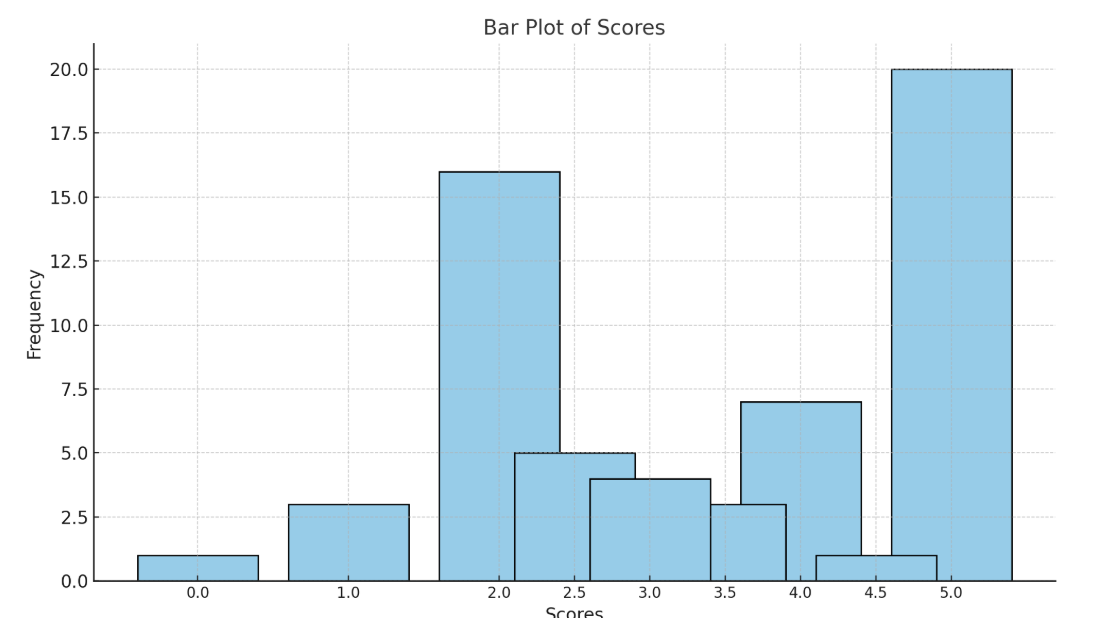
\includegraphics[width=0.5\textwidth]{images/sec5_scores.png}
\end{figure}
\footnotesize 
Great job to 1/3 of the class!
\vfill 
Thoughts if your scores are lower than you want:
\begin{itemize}
\item \textbf{Strategy} - Read \textit{actively}. Try to work out examples on own while reading
\item \textbf{Time} - Can you increase the time you spend on the reading? 
\item \textbf{Patience and persistence} - You may still be adjusting to mathematical thinking (and/or the quiz formats). Hang in there. Play the long game. 
	\begin{itemize}
	\footnotesize 
	\item Each reading quiz is less than 1\% of your total grade. You just need to catch on eventually. 
	\item The material will be retested (problems quiz and final), and that carries about \textit{twice} as much weight.
	\end{itemize}
\item \textbf{Recruit help} - Get help from me, Fatima (TA), Kelly Joyce (tutor), or elsewhere.
\end{itemize}

\end{frame}

%
%\begin{frame}{General announcements}
%\begin{itemize}
%\item Problems quizzes
%\item Handwriting.
%\item "why is 90\% of your class not teaching?" %
%\end{itemize}
%	
%\end{frame}





\begin{frame}[standout]

\alert{Sec. 6 (counterexample) group work!}
\vfill
Students are randomly assigned into groups of 3 on the next slide.
\vfill 
Each group gets $\half$ of a white board.
\vfill
If the  $\half$ white board is inconvenient, feel free to write on a window! 
\end{frame}

\begin{frame}
\footnotesize
Group 1: joseph.mergenthaler,pendleton.johnston,blake.leone\\
Group 2: connor.yetter,jacob.ketola,mason.barnocky\\
Group 3: michael.oswald,carsten.brooks,connor.graville\\
Group 4: emmeri.grooms,luka.derry,ryan.barrett2\\
Group 5: connor.mizner,kaden.price,anthony.mann\\
Group 6: nolan.scott1,bridger.voss,jack.fry\\
Group 7: lynsey.read,yebin.wallace,ethan.johnson18\\
Group 8: william.elder1,colter.huber,sarah.periolat\\
Group 9: john.fotheringham,jonas.zeiler,nicholas.harrington1\\
Group 10: peyton.trigg,tyler.broesel,micaylyn.parker\\
Group 11: jakob.kominsky,james.brubaker,alexander.knutson\\
Group 12: devon.maurer,jett.girard,samuel.mosier\\
Group 13: samuel.rollins,cameron.wittrock,jacob.ruiz1\\
Group 14: caitlin.hermanson,conner.reed1,owen.obrien\\
Group 15: julia.larsen,reid.pickert,alexander.goetz\\
Group 16: zeke.baumann,jacob.shepherd1,jeremiah.mackey\\
Group 17: evan.schoening,griffin.short,joseph.triem\\
Group 18: samuel.hemmen,delaney.rubb,derek.price4\\
Group 19: adam.wyszynski,carver.wambold,justice.mosso\\
Group 20: jada.zorn,lucas.jones6,timothy.true\\
Group 21: matthew.nagel,luke.donaldson1,peter.buckley1\\
Group 22: aaron.loomis,evan.barth,tristan.nogacki, erik.moore3
\end{frame}


\begin{frame}{Group exercises}
\begin{enumerate}
	\item Disprove: If $a$ and $b$ are integers with $a|b$, then $a \leq b$.
	\item Disprove: If $p$ and $q$ are prime, then $p+q$ is composite.
	\item Disprove: An integer $x$ is positive if and only if $x+1$ is positive.
	\item What does it mean for an if-and-only-if statement to be false? What properties should a counterexample for an if-and-only-if statement have?
\end{enumerate}

\vfill  \vfill 
(Optional.) If you have extra time, you might try these for extra practice:
\vspace{-0.5cm}
\begin{enumerate}
	\item[a.] Disprove: If $a$,$b$, and $c$ are positive integers with $a|bc$, then $a|b$ or $a|c$.
	\item[b.] Disprove: If $p$ is prime, then $2^p-1$ is also prime.
\end{enumerate}

\end{frame}


\begin{frame}{Group exercise \#1: Solution}

\textbf{Problem.} Disprove: If $a$ and $b$ are integers with $a|b$, then $a \leq b$.
\vfill 

\textbf{Solution (longer).} Let $a=5$ and $b=-5$. We will show that for this choice of $a$ and $b$, the hypothesis holds (i.e. $a|b$), but the conclusion doesn't (i.e. $a>b$).  By definition of divisibility, $a|b$ means that there is an integer $c$ such that $ac =b$. In this case, we need to show that there is an integer $c$ such that  $5c=-5$.  Indeed, the equation holds for $c=-1$.  Therefore, $b|a$, and the hypothesis holds.  However, clearly $a>b$, and so the conclusion fails. 
\vfill 
\textbf{Solution (shorter).} Let $a=5$ and $b=-5$. We will show that the hypothesis holds (i.e. $5|-5$), but the conclusion doesn't (i.e. $5>-5$).  To verify the hypothesis $5|-5$, note that there is an integer $c=-1$ such that  $5c=-5$.  We immediately see that $5>-5$, and so the conclusion fails.
\vfill 
\textbf{Remark.} In here and the following solutions , I provide longer solutions to clarify the logic for students who are struggling. However, in practice, feel free to provide shorter solutions, such as the one above.
\end{frame}


\begin{frame}{Group exercise \#2: Solution}

\textbf{Problem.} Disprove: If $p$ and $q$ are prime, then $p+q$ is composite.
\vfill 

\textbf{Solution (longer).}  Let $p=2$ and $q=3$. We will show that for the counterexample, the hypothesis holds (i.e. $2$ and $3$ are prime), but the conclusion doesn't (i.e. $r=2 + 3 = 5$ is not composite).  By definition of prime, an integer $s$ is prime if $s>1$ and the only positive divisors of $s$ are $1$ and $s$.   When $p=2$, we have that $2>1$ and the only positive divisors are $2$ and $1$, hence it is prime.  A similar statement shows that $q$ and $r$ are prime.  Hence, $p$ and $q$ are prime, and the hypothesis holds.  Moreover, $r$ is prime, and therefore not composite, and so the conclusion fails.   
\end{frame}


\begin{frame}{Group exercise \#3: Solution}

\textbf{Problem.} An integer $x$ is positive if and only if $x+1$ is positive.
\vfill 

\textbf{Solution (longer).}  Let $A$ be the proposition that an integer $x$ is positive, and $B$ be the proposition that $x+1$ is positive.  We can show that $A \iff B$ fails by showing that $B \implies A$ fails.   We show that there exists a case where $B$ is true, but $A$ is false.  In particular, take $x=0$. Then $B$ is true (since $x+1=1$ is positive), but $A$ fails (since $x=0$ is not positive.)   
\end{frame}

\begin{frame}{Group exercise \#4: Solution}

\textbf{Problem.} What does it mean for an if-and-only-if statement to be false? What properties should a counterexample for an if-and-only-if statement have?
\vfill 

\textbf{Solution.} Recall from the group exercises of Sec. 4 (Theorems) that $A \iff B$ is identical to $(A \implies B) \, \texttt{and} \, (B \implies A)$.  Hence, we can show that $A \iff B$ fails by showing that either $A \implies B$ fails or $B \implies A$ fails.  (For more information on this strategy, see the group exercise on DeMorgan's law in Sec. 7, Boolean Algebra.)
\end{frame}

\end{document}
